% https://www.overleaf.com/learn

\documentclass{article}
\usepackage{layout}
\usepackage[T1]{fontenc} 
\usepackage[italian]{babel}
\usepackage{hyphenat}
\usepackage{graphicx}
\usepackage{listings}
\usepackage{xcolor}
\usepackage{hyperref}

\hypersetup{
    colorlinks=true,
    linkcolor=blue,
    filecolor=magenta,      
    urlcolor=cyan
    }

\usepackage{geometry}
\setlength{\textheight}{640pt}
\geometry{
  a4paper,
  % total={170mm,257mm},
  % left=20mm,
  top=30mm,
  bottom=30mm,
}
\definecolor{codegreen}{rgb}{0,0.6,0}
\definecolor{codegray}{rgb}{0.5,0.5,0.5}
\definecolor{codepurple}{rgb}{0.58,0,0.82}
\definecolor{backcolour}{rgb}{0.95,0.95,0.92}

\lstdefinestyle{mystyle}{
    backgroundcolor=\color{backcolour},   
    commentstyle=\color{codegreen},
    keywordstyle=\color{magenta},
    numberstyle=\tiny\color{codegray},
    stringstyle=\color{codepurple},
    basicstyle=\ttfamily\footnotesize,
    breakatwhitespace=false,         
    breaklines=true,                 
    captionpos=b,                    
    keepspaces=true,                 
    numbers=left,                    
    numbersep=5pt,                  
    showspaces=false,                
    showstringspaces=false,
    showtabs=false,                  
    tabsize=2
}

\title{Progetto Esame Algorithmic Game Theory}
\author{Paola Guarasci --- mat 231847}
\date{\today}
\lstset{style=mystyle}

% \hyphenation{mate-mati-ca recu-perare}

\begin{document}
\maketitle

%%%%%%%%%%%%%%%%%%%%%%
%%%  Prima parte  %%%%
%%%%%%%%%%%%%%%%%%%%%%

\section*{Descrizione}
\paragraph*{Scenario iniziale}
Il problema riguarda la selezione di un sottoinsieme di utenti all'interno di un più ampio gruppo di utenti che dovranno effettuare un tour tra alcune città. Inoltre bisogna stabilire il costo da addebitare a ciascun utente.
\paragraph*{Input}
L'algoritmo in ingresso si aspetta una lista di tipi, uno per ogni utente. Il tipo rappresenta la località preferita di ogni agente. È stata introdotta una semplificazione riguardo al problema posto originariamente: gli agenti non forniscono una lista di preferenze bensì una sola preferenza di cui ci si può fidare poiché è stato adottato un meccanismo di scelta basato sul mento massimo che ogni agente è disposto a effettuare. Quindi, poiché dell'affermazione sul pagamento ci si può fidare, allora si è deciso di usare questo criterio come discriminante per quanto riguarda l'inserimento del singolo agente nel sottoinsieme travellers, cioè l'insieme dei viaggiatori.
In fase di test dell'algoritmo l'input è stato generato casualmente, rispettando i limiti di cardinalità dell'insieme delle località (nessun agente può preferire una località che non esiste).
\paragraph*{Grafo}
Le località sono rappresentate da un grafo pesato non orientato. Ogni località, ovvero ogni nodo, è connessa con tutte le altre località. I pesi sugli archi indicano la distanza in chilometri tra i due nodi alle estremità di ogni arco.
\begin{figure}[h]
  \centering
  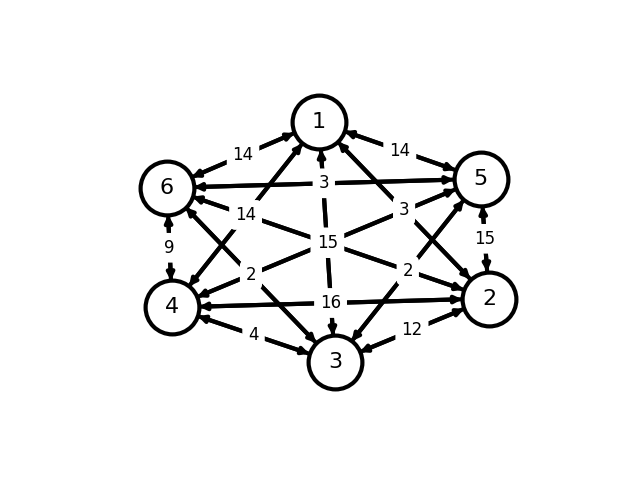
\includegraphics[width=0.50\textwidth]{img/graphTot.png}
  \caption{Grafico generale delle località}\label{fig:graphTot.png}
\end{figure}
Il calcolo del percorso ottimale e del suo costo è stato modellato usando l'algoritmo di Dijkstra e risolvendo il problema del Commesso Viaggiatore. Per far ciò ci siamo avvalsi di una ottima libreria in Python per la manipolazione di grafi\footnote{NetworkX, rilasciata con licenza BSD (Open Source) \url{https://networkx.org/}}. La funzione di libreria \verb|approx.greedy_tsp(graph)| prende in input un grafo (o porzione di esso) e ne calcola il cammino hemiltoniano.
Per avere il costo del cammino la formula usata è la seguente:
\begin{lstlisting}[language=Python]
cost = sum(graph[n][nbr]["weight"] for n, nbr in nx.utils.pairwise(cycle))
\end{lstlisting}
Il grafo è modellato come una lista di tuple di archi con tre valori: nodo di partenza, nodo di arrivo, peso.
I nodi sono inferiti dalla lista di archi.
\paragraph*{Output}
In uscita si ottiene una lista di viaggiatori e una lista di località selezionate.
\paragraph*{Meccanismo}
Il core del progetto è l'algoritmo di selezione degli agenti. Per ogni agente si valuta la possibilità d'inclusione nel gruppo di viaggiatori, i \verb|travellers|, usando la seguente strategia di selezione:
\begin{itemize}
  \item Se è stato raggiunto il limite massimo di capienza della macchina, non fare niente.
  \item Altrimenti, valuta il costo del viaggio tra le località già selezionate e quella nuova preferita dall'agente.
  \item Se il costo è accettabile e non si superano i vincoli in termini di chilometri massimi, allora inserisci l'agente nel gruppo viaggiatori e la nuova località nel gruppo di località selezionate.
  \item Infine, per ogni utente già inserito nel gruppo viaggiatori valuta se il nuovo costo del viaggio è accettabile e se non dovesse esserlo elimina l'agente dal gruppo viaggiatori. Elimina anche la località scelta se non è preferita da nessun agente rimasto nel gruppo viaggiatori.
\end{itemize}
È un meccanismo diretto la cui modalità di selezione di ogni singolo viaggiatore consente di essere sicuri riguardo l'applicazione di strategie dominanti da parte dei vari agenti, poiché non avviene tramite utilità, che per definizione (vedi traccia) non è affidabile, ma avviene in base al pagamento che ogni agente è disposto a fare (considerato affidabile).
Il costo fisso per ogni agente è calcolato dividendo la somma per la cardinalità dell' insieme \verb|travellers|.
\paragraph*{Esempio di output}
Ecco un esempio di output: la prima riga sono gli utenti selezionati, la seconda riga sono le località selezionate, poi costo di viaggio totale e costo di viaggio pro capite.
\begin{lstlisting}[language=bash]
$ python src/agt.py
{(4, 2, 14), (6, 60, 12), (3, 85, 10), (3, 14, 13), (5, 20, 16)}
{3, 4, 5, 6}
Num Viaggiatori:  5
Costo viaggio:  15.0
Costo viaggio pro capite:  3.0
\end{lstlisting}

\begin{figure}[h]
  \centering
  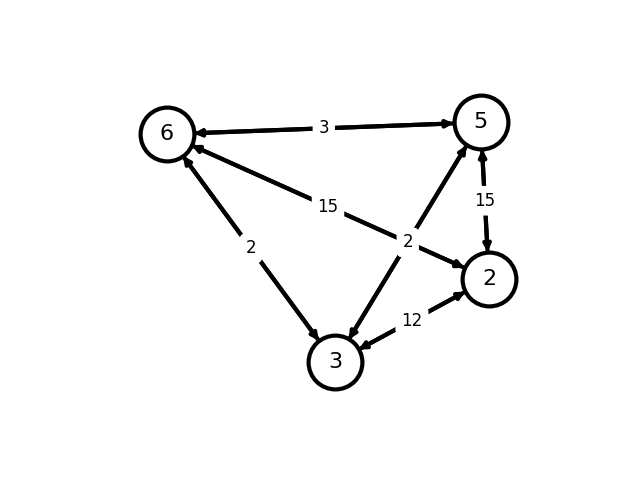
\includegraphics[width=0.50\textwidth]{img/graphOutput.png}
  \caption{Sotto grafo con località selezionate per il tour}\label{fig:graphOutput.png}
\end{figure}
\clearpage
\pagebreak

%%%%%%%%%%%%%%%%%%%%%%
%%% Seconda parte %%%%
%%%%%%%%%%%%%%%%%%%%%%

\section*{Implementazione}
\lstinputlisting[language=Python]{../src/agt.py}
\end{document}